\chapter{硅基反射微环的光调制器}
纯硅基调制器的进展我们已经在第一章\ref{pure_simodulator}中有所分析。硅基光调制器目前都采用调节波导折射率,从而改变谐振腔的谐振峰或者,或者改变马赫曾德两臂的相位实现调制。谐振腔型硅基光调制器,可以采用微环或者光子晶体结构。这类光调制器具有尺寸小,速度快的特点,但是光学带宽受到谐振峰漂移量的限制。如果采用热调节微环谐振峰的位置,那么只有10~nm左右的漂移量。而硅基马赫曾德型光调制器具有光学带宽大,速度大的特点,但是调制区尺寸大。目前硅基微弱的等离子色散效应,至少需要500~$\mu m$的臂长才能调节$\Pi$的相位变化。

在本章中我们分析在微环内引入可调的反射镜,从而可以调制输出波导光的强度。首先我们对微环内有反射进行了理论分析。接下来我们在微环内加工光栅,研究不同反射率下,微环透射谱的变化。随后,我们分析可调反射镜的性质。最后我们设计了在微环中集成可调反射镜,实现光的强度调制。
\section{微环内反射的理论分析}
微环内反射对微环性能的影响可以时域或者频域为切入点进行分析。以频域为切入点,需要采用传输矩阵模型\cite{yariv2006photonics}。而以时域为切入点,需要用时变的微分方程来分析\cite{haus1984waves}。由于频域模型下的传输矩阵模型需要考虑微环内部反射的具体结构,以及具体的工作波长,因此更适用于设计。而时域中的时变微分方程则更适合分析反射对微环的动态和静态进行分析。下面我们首先介绍基于时变的微分方程法分析反射对微环透射谱的影响\cite{haus1984waves,Li2016design,little1997microring}。
\begin{figure}[htb]
	\centering
	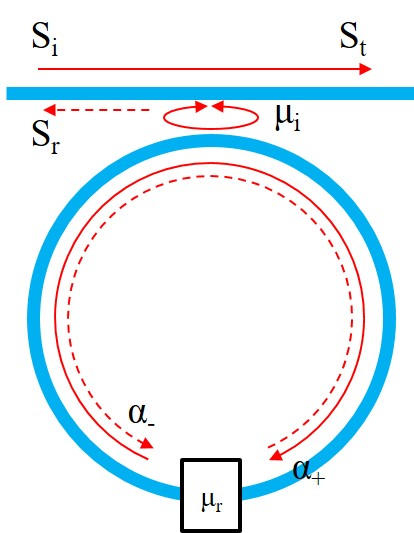
\includegraphics[width=6cm]{./Pictures/chapt5_ring_reflector_structure.jpg}
	\caption{在时序耦合模式理论(tCMT)下,有内部反射的微环模型。其中正向传播的能量$\alpha_+$和反向传播的能量$\alpha_-$,在反射处相互耦合}
	\label{chapt5_ring_reflector_structure}
\end{figure}
基于时变的微分方程法又称作时序耦合模式理论(Temporal Coupled Mode Theory, tCMT)。当微环内部有反射时,微环内部就会有两个方向传播的光模式,如图\ref{chapt5_ring_reflector_structure}所示。我们根据其传播的方向,将其正向传播的幅值记为$\alpha_+$,将反向传播的幅值记为$\alpha_-$。而$|\alpha_+|^2$和$|\alpha_-|^2$表示正向传播和反向传播模式的能量。当微环中有反射时,这两个模式在反射处相互耦合,从而影响了微环的正常输出光谱,使其消光比发生变化,甚至谐振模式产生了劈裂。如果用tCMT方程描述这种情况就如公式\ref{Equ:alpha_ccw},公式\ref{Equ:alpha_cw}和公式\ref{Equ:St_Sr}所示\cite{Li2016design}。
\begin{equation}
\label{Equ:alpha_ccw}
\frac{d\alpha_+}{dt}=j\omega_0\alpha_+-\left(\frac{1}{\tau_i}+\frac{1}{\tau_l}\right)\alpha_+-j\mu_iS_i-j\mu_r\alpha_-
\end{equation}
\begin{equation}
\label{Equ:alpha_cw}
\frac{d\alpha_-}{dt}=j\omega_0\alpha_--\left(\frac{1}{\tau_i}+\frac{1}{\tau_l}\right)\alpha_--j\mu_r^*\alpha_-
\end{equation}
\begin{equation}
\label{Equ:St_Sr}
S_t = S_i-j\mu_i\alpha_+ ~~~~~~~~~~~~ S_r = -j\mu_i\alpha_-
\end{equation}
其中$\omega_0$是微环的谐振频率。$S_i$表示输入光的振幅。$1/\tau_i$表示微环中光场耦合到波导导致的能量衰减率。$1/tau_l$表示微环中的光场由于微环本身弯曲,材料等损耗$\alpha_l$导致的能量衰减率。$\mu_i$是波导和微环的波导耦合强度。$\mu_r$是$\alpha_+$和$\alpha_-$的反射耦合强度。其中,波导耦合强度$\mu_i$与衰减率$\tau_i$,损耗系数$\alpha_l$与衰减率$\tau_l$,反射耦合强度$\mu_r$与光场反射率$r$的关系分别如公式\ref{Equ:mu_tau}所示\cite{little1997microring}。
\begin{equation}
\label{Equ:mu_tau}
\mu_i^2=k_i^2\frac{c}{n_gL}=\frac{2}{\tau_i}~~~~~~~~~~~~\alpha_l^2\frac{c}{n_gL}=\frac{2}{\tau_l}~~~~~~~~~~~~\mu_r^2=r^2\frac{c}{n_gL}^2
\end{equation}
其中$c$是真空中的光速,$n_g$是波导的群折射率,$L$是微环的周长。通过解公式\ref{Equ:alpha_ccw}、公式\ref{Equ:alpha_cw}和公式\ref{Equ:St_Sr},我们可以获得波导输出光场$S_i$与输入光场$S_i$的关系如公式\ref{Equ:St}所示。
\begin{equation}
\label{Equ:St}
\frac{S_t}{S_i}=1-\frac{1}{\tau_i}\left(\frac{1}{j(\omega-\omega_1)+(1/\tau_i+1/\tau_l)} + \frac{1}{j(\omega-\omega_2)+(1/\tau_i+1/\tau_l)}\right)
\end{equation}

可以看到,此时输出光谱需要用两个洛仑兹线形(Lorentzian-shape)进行拟合,而传统的微环,只需要一个洛仑兹线线。两个洛仑兹线形的中心频率分别为$\omega_1 = \omega_0+|\mu_r|$,$\omega_2=\omega_0-|\mu_r|$。中心频率的偏移量正比于微环的反射耦合强度$\mu_r$,也就是中间反射器的反射强度$r$。在两个谐振频率出的透射率$P_r$如公式\ref{Equ:Pr}所示。
\begin{equation}
\label{Equ:Pr}
P_r = \left|\frac{S_t}{S_i}\right|^2_{\omega = \omega_1~or~\omega_2}= \left(\frac{\alpha_l^2}{k_i^2+\alpha_l^2}\right)^2+\frac{(k_i^4-2k_i^2\alpha_l^2)}{(k_i^2+\alpha_l^2)^2+16r^2}
\end{equation}
当$r=0$时,公式\ref{Equ:Pr}就变成了普通微环的谐振频率处的透射率:
\begin{equation}
\label{Equ:Pr_no_r}
P_r=\left(\frac{\alpha_l^2-k_i^2}{k_i^2+\alpha_l^2}\right)^2
\end{equation}
当$k_i = \alpha_l$时,微环处于临界工作点,$k_i$成为临界耦合系数$k$。此时,普通微环在谐振频率处的透射率达到最小值0。而当微环内有反射时,谐振峰处的透射谱将于反射率$r$有关,如公式\ref{Equ:Pr_critical_r}所示。微环在谐振峰处的消光比我们采用公式\ref{Equ:RingER}的定义。
\begin{equation}
\label{Equ:RingER}
ER_{ring}=-10 \times log_{10}(Pr)
\end{equation}
\begin{equation}
\label{Equ:Pr_critical_r}
P_r=\frac{1}{4}-\frac{k_i^4}{4k_i^2+16r^2}
\end{equation}
\begin{figure}[htb]
	\centering
	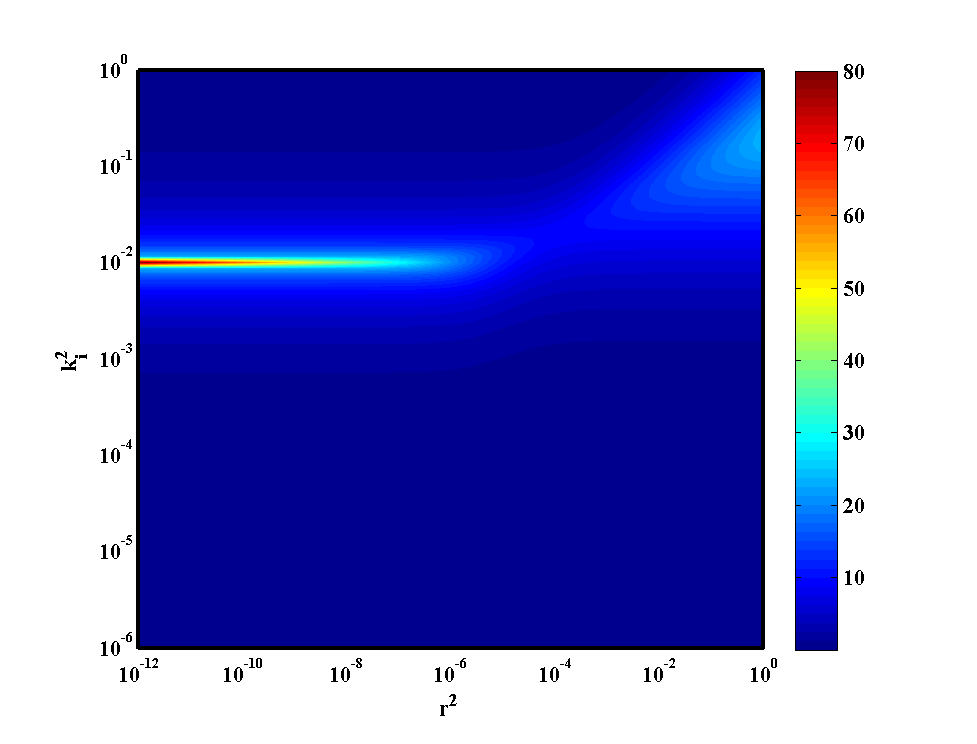
\includegraphics[width=12cm]{./Pictures/chapt5_r_k_Ex_alpha1e-2.eps}
	\caption{当微环损耗$\alpha_l^2= 10^{-2}$时,谐振峰处的消光比与耦合系数$k_i^2$,内部反射率$r^2$的关系}
	\label{chapt5_r_k_Ex_alpha1e-2}
\end{figure}
\begin{figure}[htb]
	\centering
	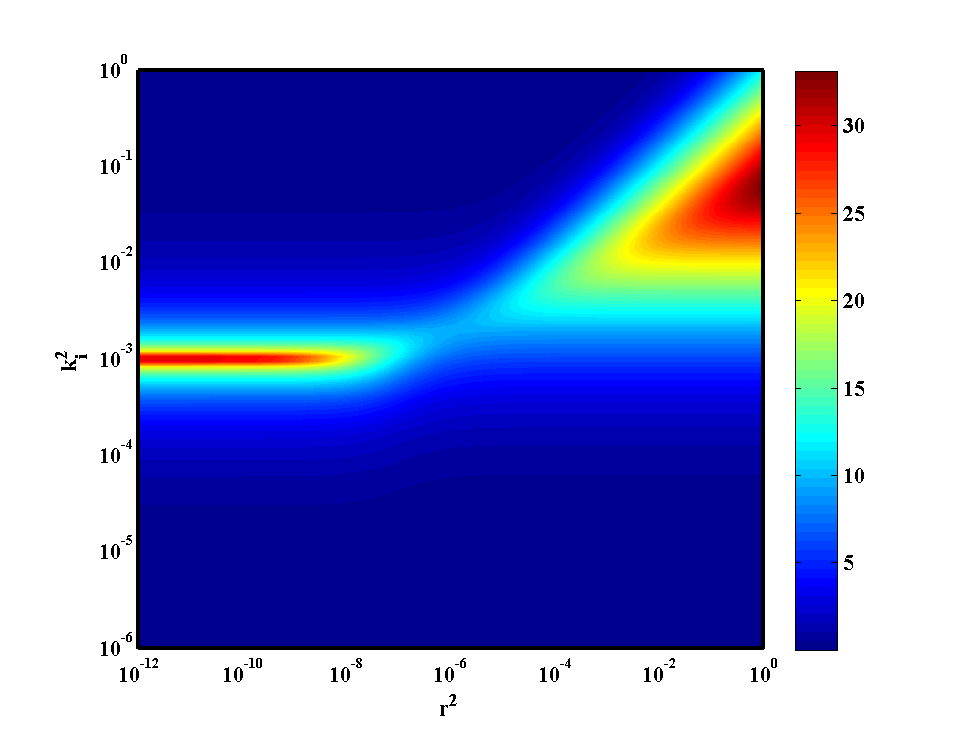
\includegraphics[width=12cm]{./Pictures/chapt5_r_k_Ex_alpha1e-3.eps}
	\caption{当微环损耗$\alpha_l^2= 10^{-3}$时,谐振峰处的消光比与耦合系数$k_i^2$,内部反射率$r^2$的关系}
	\label{chapt5_r_k_Ex_alpha1e-3}
\end{figure}
\begin{figure}[htb]
	\centering
	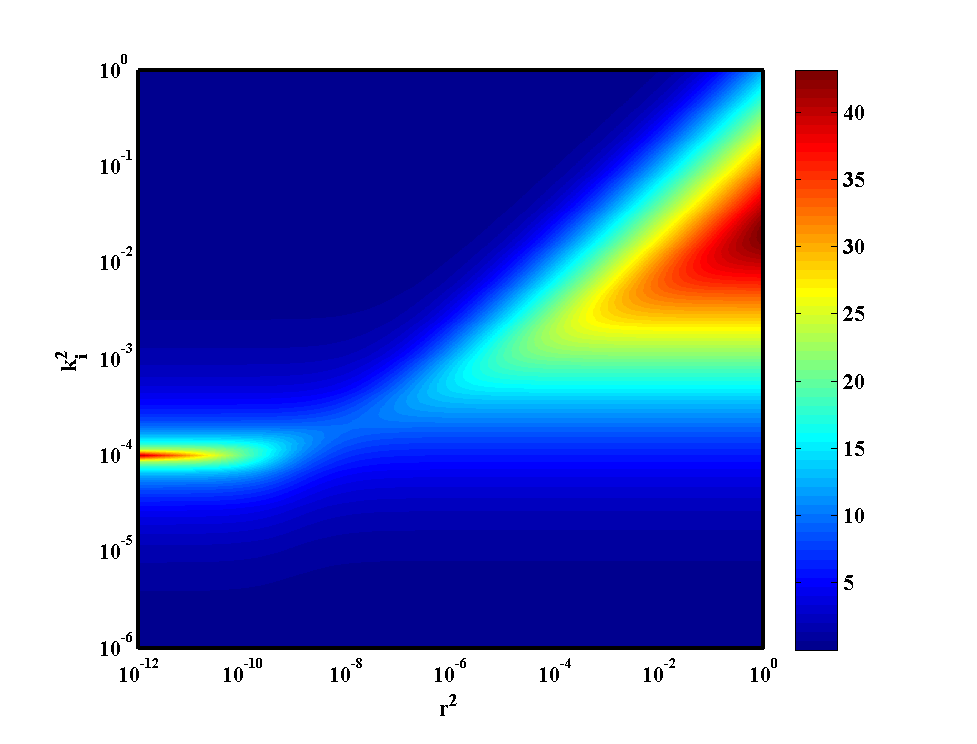
\includegraphics[width=12cm]{./Pictures/chapt5_r_k_Ex_alpha1e-4.eps}
	\caption{当微环损耗$\alpha_l^2= 10^{-4}$时,谐振峰处的消光比与耦合系数$k_i^2$,内部反射率$r^2$的关系}
	\label{chapt5_r_k_Ex_alpha1e-4}
\end{figure}
图\ref{chapt5_r_k_Ex_alpha1e-2},\ref{chapt5_r_k_Ex_alpha1e-3},\ref{chapt5_r_k_Ex_alpha1e-4}展示了,在不同损耗$\alpha_l$的微环中,$k_i$,$r$对谐振频率处的消光比的影响。从图\ref{chapt5_r_k_Ex_alpha1e-2}可以看到,当微环的损耗很大($\alpha_l^2 = 10^{-2}$)时,微环内部存在微弱的反射时($r^2<10^{-7}$),对$k_i$与消光比的关系影响很弱,依旧是在$k_i=\alpha_l$时存在最大的消光比。不过此时,临界耦合处的消光比,随着反射率的增大而减弱。当微环内部存在的反射率继续增大时,$k_i$的变化对消光比的影响逐渐弱。而且谐振峰消光比最大处满足的条件不再是$k_i = \alpha_l$,而是$k_i > \alpha_l$,并且随着$r$的增加对应的$k_i$继续增大。

当微环内部损耗降低到$\alpha_l^2 = 10^{-3}$时,从图\ref{chapt5_r_k_Ex_alpha1e-3}可以看到,微环对内部的反射敏感。只有当$r^2<10^{-8}$时,微环才能保持原先的$k_i$与消光比的关系。当微环内部的反射率继续增加到$r>10^{-4}$时,谐振峰的消光比最大时的$k_i$也是随着$r$的增加而增大。并且相比于$r^2<10^{-8}$时,高的消光比只存在很窄的$k_i\approx k_i$区域,而当$r^2>10^{-2}$,高的消光比对应更宽的$k_i$区域。

当微环的内部损耗继续降低到$\alpha_l^2=10^{-4}$时,从图\ref{chapt5_r_k_Ex_alpha1e-4}可以看到,微环对内部反射更加敏感。在临界耦合处的微环只需要引入极小的反射{$r^2\approx 10^{-10}$},消光比就会有很大的改变。而当$r>10^{-6}$时,谐振峰的消光比最大时对应的$k_i$和$r$的变化几乎成线性关系。$r^2>10^{-2}$时,高的消光比存在的区域比之前高损耗的情况下,面积更大。

利用微环内反射引起反射谱变化的现象,之前研究人员已经在超低损耗微盘中,利用微小颗粒附着微盘引起微环内部微小反射,从而使实现检测半径只有30~nm纳米颗粒\cite{zhu2010chip}。而对于当微环内部反射率很大时,高消光比的微环对耦合系数不敏感的现象,我们可以用于实现工艺容差大的光波长滤波器\cite{qiangsheng2015fsr}。

我们在本论文中,我们将探讨调制微环内部反射率从而实现光调制器。不过下面我们先将对这个理论现象进行实验的验证。
\section{微环内反射的设计与实验}
\subsection{微环内反射的结构设计和仿真}
\subsection{微环内反射的制作和实验结果}
\section{硅基可调反射镜的设计}
\section{硅基可调反射镜的微环调制器的设计}